\chapter{Constructions}

\section{Introduction}

In this chapter, we present diagrammed proofs of lethal sets that percolate at the lower bound. The proofs are organized by the thickness of the grid. Many of the constructions in the following sections belong to infinite families of either optimal or perfect sets. In this case, we shall examine the grids by region, and observe that certain regions can be expanded to arbitrarily large sizes using mathematical induction. 

We shall call a thickness \emph{semi-complete} if all divisibility cases are optimal.

\section{Useful lemmas and observations}

We shall see that similar patterns and structures appear with some regularity in optimal sets. These structures always infect entire regions, and it will be helpful to recognize them within larger grids when they appear. 

\section{Thickness 2}

\begin{con}
All $(a,b,2)$ grids with $a,b \in \{0,3\} \pmod 6$ and $a \neq b \pmod 6$ are perfect. 
\end{con}

\begin{proof}
We proceed by induction. For the base case, consider the grid $(6,9,2)$ (figure \ref{fig:6x9x2}).
\end{proof}

\begin{figure}[]
\centering
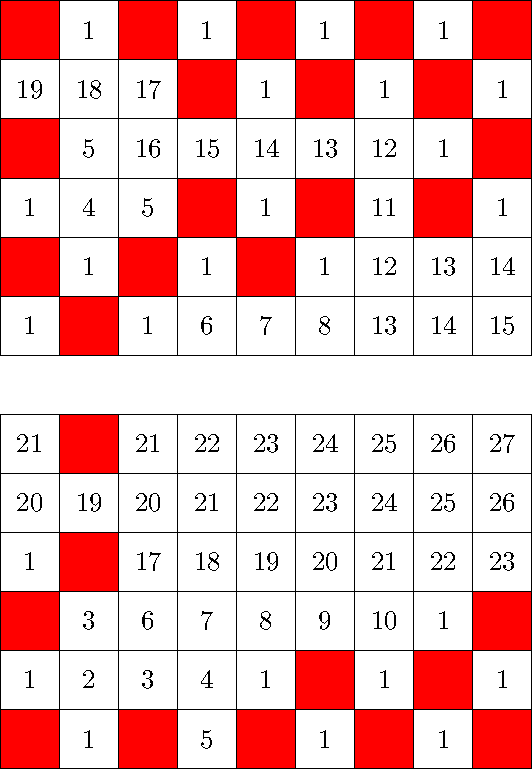
\includegraphics[width=\textwidth]{figures/4/6x9x2_numbered_heatmap.pdf}
\caption{}
\label{fig:6x9x2}
\end{figure} 

\begin{figure}[]
\centering
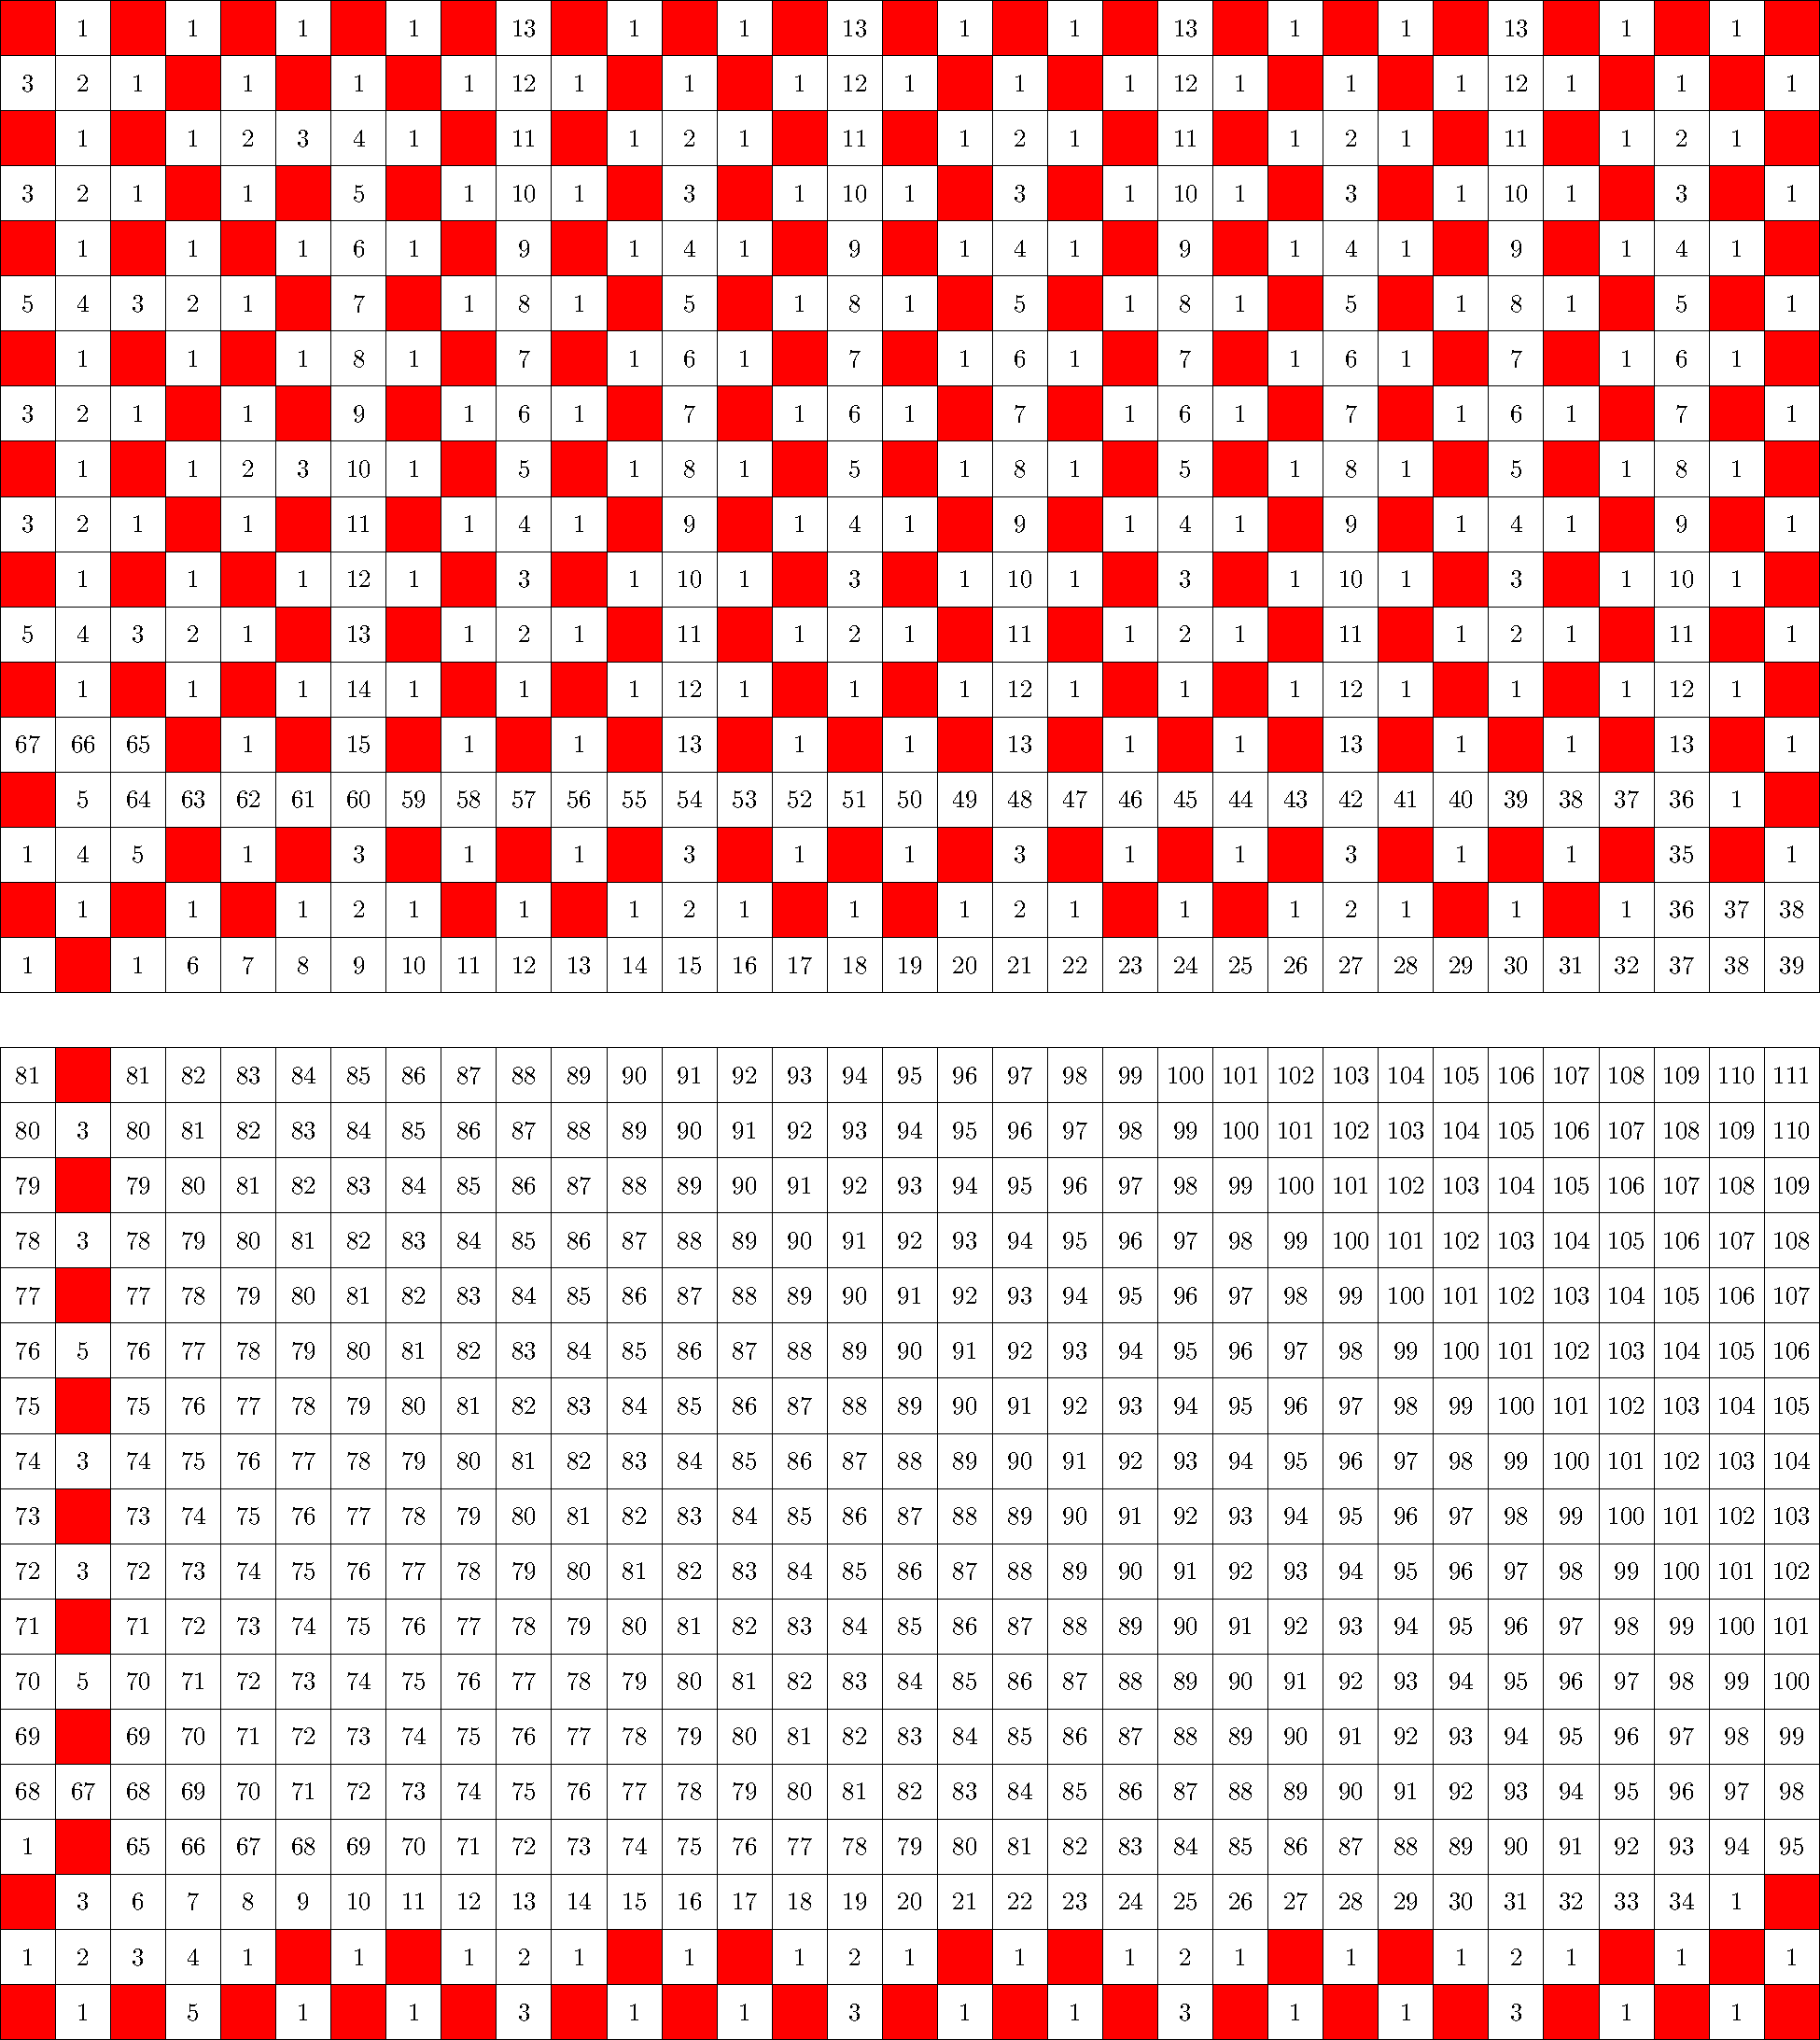
\includegraphics[width=\textwidth]{figures/4/18x33x2_numbered_heatmap.pdf}
\caption{}
\label{fig:6x9x2}
\end{figure} 
